\documentclass[12pt,a4paper,twoside,openright,titlepage,final]{article}
\usepackage{fontspec}
\usepackage{amsmath}
\usepackage{amsfonts}
\usepackage{amssymb}
\usepackage{makeidx}
\usepackage{graphicx}
\usepackage[hidelinks,unicode=true]{hyperref}
\usepackage[spanish,es-nodecimaldot,es-lcroman,es-tabla,es-noshorthands]{babel}
\usepackage[left=3cm,right=2cm, bottom=4cm]{geometry}
\usepackage{natbib}
\usepackage{microtype}
\usepackage{ifdraft}
\usepackage{verbatim}
\usepackage[obeyDraft]{todonotes}
\ifdraft{
	\usepackage{draftwatermark}
	\SetWatermarkText{BORRADOR}
	\SetWatermarkScale{0.7}
	\SetWatermarkColor{red}
}{}
\usepackage{booktabs}
\usepackage{longtable}
\usepackage{calc}
\usepackage{array}
\usepackage{caption}
\usepackage{subfigure}
\usepackage{footnote}
\usepackage{url}
\usepackage{tikz}
\tikzset{
  treenode/.style = {shape=rectangle, rounded corners,
                     draw, align=center,
                     top color=white, bottom color=blue!20},
  root/.style     = {treenode, font=\Large, bottom color=red!30},
  env/.style      = {treenode, font=\ttfamily\normalsize},
  dummy/.style    = {circle,draw}
}

\setsansfont[Ligatures=TeX]{texgyreadventor}
\setmainfont[Ligatures=TeX]{texgyrepagella}

%*******************************************************
%                 NO MODIFICAR
\newcommand*{\FSfont}[1]{%
  \fontencoding{T1}\fontfamily{#1}\selectfont}

\newlength{\tpheight}\setlength{\tpheight}{0.9\textheight}
\newlength{\txtheight}\setlength{\txtheight}{0.9\tpheight}
\newlength{\tpwidth}\setlength{\tpwidth}{0.9\textwidth}
\newlength{\txtwidth}\setlength{\txtwidth}{0.9\tpwidth}
\newlength{\drop}
%*******************************************************

% Crea una portada con los siguientes parámetros
%
% #1 : Título 
% #2 : Subtítulo
% #3 : Subsubtítulo
% #4 : Autor(es)
% #5 : Lugar
%

\newcommand*{\portada}[5]{
\begin{titlepage}
\begingroup
\vspace*{1cm}
\drop = 0.2\txtheight
\centering
\vfill
{\Huge \scshape #1}\\[\baselineskip]
{\Large \textbf{#2}}\\[\baselineskip]
{\Large \scshape #3}\\[\baselineskip]
\vspace*{0.3cm}
{\large \textit{#4}}\\[0.5\drop]

\includegraphics[scale=0.35]{./imagenes/logoURJC.jpg}
\vspace*{1.5cm}

{\large \scshape #5, \today} \par
\begin{center}
\end{center}
\vfill\null
\endgroup
\end{titlepage}
}
 %*****************************************************
 


\author{José Ignacio Escribano}

\title{Caso práctico II}

\setlength{\parindent}{0pt}

\begin{document}

\pagenumbering{alph}
\setcounter{page}{1}

\portada{Caso Práctico II}{Modelización y tratamiento de la incertidumbre}{Probabilidades y variables aleatorias}{José Ignacio Escribano}{Móstoles}

\listoffigures
\thispagestyle{empty}
\newpage

\tableofcontents
\thispagestyle{empty}
\newpage


\pagenumbering{arabic}
\setcounter{page}{1}

\section{Introducción}

En este caso práctico resolveremos distintos problemas relativos a variables aleatorias, tanto discretas como continuas. Las dos primeras tareas se refieren a las primeras variables, y las dos últimas, a las segundas. En las cuatro tareas calcularemos probabilidades, realizaremos distintos tipos gráficos y responderemos a las preguntas planteadas.

\section{Resolución del caso práctico}



\subsection{Tarea IV}

El beneficio de cada inversión viene dado por la diferencia entre los beneficios netos y la inversión (1 millón de euros). Así, por tanto, si se pierde todo lo invertido tenemos que el beneficio es -1 (los beneficios netos son cero y la inversión 1); cuando no se obtiene beneficio neto ni se pierde la inversión tenemos que los beneficios son 0 (se tiene un beneficio neto de un millón y un mi millón de inversión).\\

Si denotamos con $X_i$ al beneficio neto obtenido en la inversión $i$ con $i = 1,2,3$, tenemos que las funciones de masa vienen dadas de la siguiente forma:

\begin{equation*}
f(X_1 = x) = \begin{cases}
0.1, & \text{si } x = 5 \\
0.3, & \text{si } x = 1 \\
0.6, & \text{si } x = -1
\end{cases}
\end{equation*}

\begin{equation*}
f(X_2 = x) = \begin{cases}
0.2, & \text{si } x = 3 \\
0.4, & \text{si } x = 1 \\
0.4, & \text{si } x = -1
\end{cases}
\end{equation*}

\begin{equation*}
f(X_3 = x) = \begin{cases}
0.1, & \text{si } x = 6 \\
0.7, & \text{si } x = 0 \\
0.2, & \text{si } x = -3
\end{cases}
\end{equation*}

En la Figura~\ref{fig:funciones_masa_inversiones} se pueden ver las funciones de masa de las tres inversiones.\\ 

\begin{figure}[tbph!]
\centering
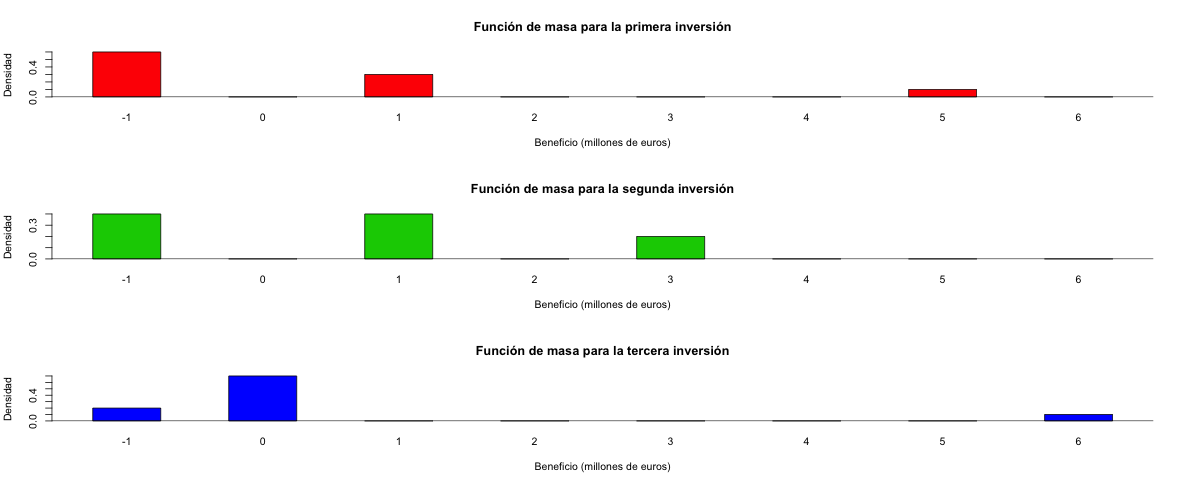
\includegraphics[width=0.9\linewidth]{imagenes/funciones_masa_inversiones}
\caption{Funciones de masa de las inversiones}
\label{fig:funciones_masa_inversiones}
\end{figure}

Calculamos la media y la varianza del beneficio de cada inversión.

\begin{align*}
E[X_1] & = \sum_{i \in \Omega_1} i\cdot f(X_1 = i) \\ & = 5 \cdot 0.1 + 1 \cdot 0.3 - 1 \cdot 0.6 \\ & = 0.2
\end{align*}

\begin{align*}
Var[X_1] & = \sum_{i \in \Omega_1} f(X_1 = i) (x_i - E[X_1])^2 \\ & = 0.1(5 - 0.2)^2 + 0.3(1-0.2)^2 + 0.6(-1 - 0.2)^2 \\ & = 3.36
\end{align*}

donde $\Omega_1 = \{-1, 1, 5\}$ es el soporte de la variable $X_1$.\\

De igual forma, se obtiene que 

\begin{align*}
E[X_2] & = 0.6 \\
Var[X_2] & = 2.24
\end{align*}

\begin{align*}
E[X_3] & = 0.4 \\
Var[X_3] & = 3.64
\end{align*}

con $\Omega_2 = \{-1, 1, 3\}$ y $\Omega_3 = \{-1, 0, 6\}$, los soportes de las variables $X_2$ y $X_3$, respectivamente.\\

Para ver la inversión más segura, calculamos la probabilidad de obtener beneficios, es decir, $P(X_i > 0)$ con $i = 1,2,3$. Así, tenemos que\\

\begin{align*}
P(X_1 > 0) & = 1 - P(X_1 \leq 0) \\ & = 1 - P(X_1 = -1) \\ & = 1 - 0.6 \\ & = 0.4
\end{align*}

\begin{align*}
P(X_2 > 0) & = 1 - P(X_2 \leq 0) \\ & = 1 - P(X_2 = -1) \\ & = 1 - 0.4 \\ & = 0.6
\end{align*}

\begin{align*}
P(X_3 > 0) & = 1 - P(X_3 \leq 0) \\ & = 1 - (P(X_3 = -1) + P(X_3 = 0)) \\ & = 1 - 0.7 - 0.2 \\ & = 0.1
\end{align*}

Teniendo en cuenta los datos de la esperanza y la varianza, y las probabilidades calculadas anteriormente, vemos que la opción más segura para obtener algún beneficio es la segunda, ya que hay 60\% de probabilidades de ganar algo de dinero con esta inversión, junto con su mayor esperanza y su menor varianza. \\

Para ver la inversión más arriesgada, calculamos la probabilidad de no perder dinero, es decir, $P(X_i \geq 0)$,

\begin{align*}
P(X_1 \geq 0) & = 1 - P(X_0 < 0) \\ & = 1 - P(X_1 = -1) \\ & = 1 - 0.6 \\ & = 0.4
\end{align*}

\begin{align*}
P(X_2 \geq 0) & = 1 - P(X_2 < 0) \\ & = 1 - P(X_2 = -1) \\ & = 1 - 0.4 \\ & = 0.6
\end{align*}

\begin{align*}
P(X_3 \geq 0) & = 1 - P(X_3 < 0) \\ & = 1 - P(X_3 = -1) \\ & = 1 - 0.2 \\ & = 0.8 
\end{align*}

La opción más arriesgada es la tercera, donde hay más probabilidades de no perder dinero, pero hay un 70\% de no ganar nada, aunque en caso de ganar, ganaremos la mayor cantidad de dinero de todas las inversiones, 6 millones de euros.\\

Calculamos la probabilidad de que la inversión más arriesgada proporcione más beneficios que la más segura, es decir, $P(X_3 > X_2)$. Tenemos, una variable bidimensional. Calculamos la función de masa conjunta $f(X_3 = x, X_2 = y) = f(X_3 = x) \cdot f(X_2 = y) \ \forall (x,y) \in \Omega_3 \times \Omega_2$, suponiendo independencia entre las variables (en principio, se puede suponer que los beneficios de una empresa no dependen de la otra). La función de masa conjunta viene dada por la siguiente tabla:

\begin{table}[htbp!]
\centering
\begin{tabular}{cccc}
\hline
$X_3$ \textbackslash $X_2$ & -1                     & 1                      & 3                      \\ \hline
-1                         & $0.2 \cdot 0.4 = 0.08$ & $0.2 \cdot 0.4 = 0.08$ & $0.2 \cdot 0.2 = 0.04$ \\ \hline
0                          & $0.7 \cdot 0.4 = 0.28$ & $0.7 \cdot 0.4 = 0.28$ & $0.7 \cdot 0.4 = 0.28$ \\ \hline
6                          & $0.1 \cdot 0.4 = 0.04$ & $0.1 \cdot 0.4 = 0.04$ & $0.1 \cdot 0.2 = 0.02$ \\ \hline
\end{tabular}
\end{table}

Tenemos que ver qué puntos de $\mathbb{R}^2$ cumplen que $X_3 > X_2$. Si representamos cada punto en el plano (Figura~\ref{fig:puntos_discreta}), vemos que los únicos que cumplen la condición anterior son $\Pi = \{(0,-1), (6,-1), (6,1), (6,3)\}$.\\

\begin{figure}[tbph!]
\centering
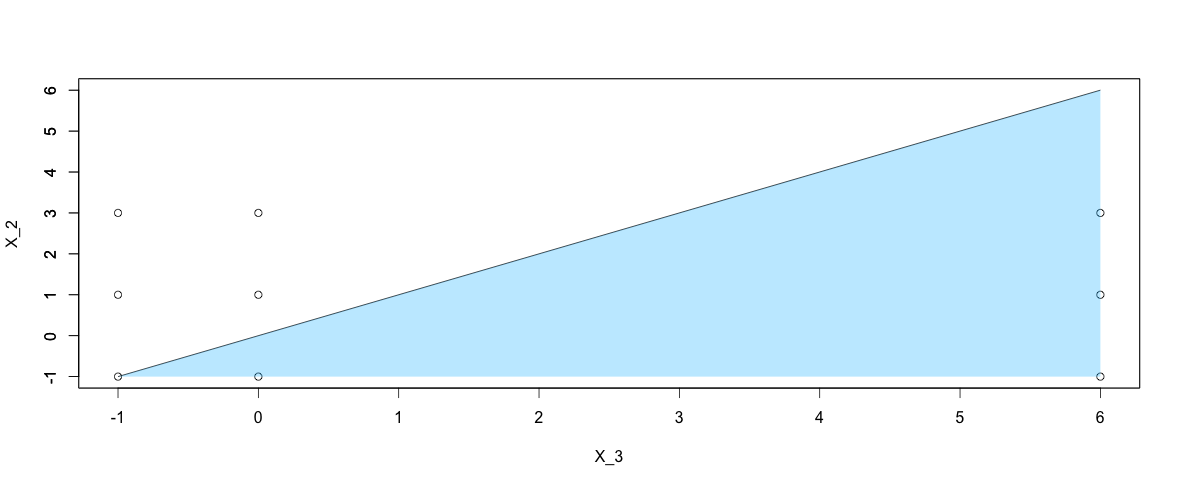
\includegraphics[width=0.9\linewidth]{imagenes/puntos_discreta}
\caption{Puntos de la función conjunta de masa}
\label{fig:puntos_discreta}
\end{figure}

Por tanto, la probabilidad pedida se calcula sumando las probabilidades de cada punto $f(x,y) \ \forall (x,y) \in \Pi$, calculadas en la tabla anterior. Esto es,

\begin{align*}
P(X_3 > X_2) & = f(0,-1) + f(6, -1) + f(6,1) + f(6,3) \\
& = 0.28 + 0.04 + 0.04 + 0.08 \\
& = 0.44
\end{align*} 

Si 10 SICAV invierten cada una un millón de euros en la empresa con más riesgos y otro millón en las empresa más segura, calculamos cuántas de ellas es de esperar que obtengan más beneficios de la inversión más arriesgada que de la más segura. Tenemos una variable aleatoria binomial con $n =10$ y $p = 0.44$, calculada en el apartado enterior. Así pues,

\begin{align*}
E[X] & = n \cdot p \\
& = 10 \cdot 0.44 \\
& = 4.4 
\end{align*}

Es decir, 4 de las 10 SICAVS obtendrán un beneficio mayor con la inversión más arriesgada que con la más segura.

\subsection{Tarea V}

Si denotamos con $X$ al número de trozos de cáscara de huevo que hay una tarta. Por el enunciado, deducimos que $E[X] = \frac{3}{2}$. Tenemos que $X \sim \mathcal{P}ois(\lambda)$. Por otro lado, la esperanza de una distribución Poisson de parámetro $\lambda$ es igual a ese mismo parámetro. Por tanto, tenemos que $\lambda = \frac{3}{2}$ y $X \sim \mathcal{P}ois(\frac{3}{2})$.

A tenor de lo anterior, el número esperado de trocitos en una tarta es $E[X] = \frac{3}{2}$.\\

La probabilidad de que no haya ningún trozo de cáscara de huevo en la tarta pedida es $P(X=0)$,

\begin{align*}
P(X=0) & = \dfrac{e^{\frac{-3}{2}} \left(\frac{3}{2}\right)^0 }{0!} \\ & = 0.2231
\end{align*}

Calculamos la probabilidad de que haya siete trozos de cáscara de huevo en una tarta, $P(X=7)$,

\begin{align*}
P(X=7) & = \dfrac{e^{\frac{-3}{2}} \left(\frac{3}{2}\right)^7}{7!} \\ & = 0.0007
\end{align*}

Por tanto, es posible que nos encontráramos una tarta con siete trozos de cáscara de huevo, aunque es muy poco probable: de cada 1000 tartas, 7 tienen siete trozos de cáscara de huevo.\\

Si pedimos 6 tartas, la probabilidad de que no haya ningún trocito en ninguna de las tartas, se calcula de la siguiente manera: tenemos una variable aleatoria $Y \sim \mathcal{B}in(n=6, p = 0.2231)$ donde $p$ lo hemos calculado en los apartados anteriores. Así, la probabilidad pedida es $P(Y = 6)$,

\begin{align*}
P(Y=6) & = \binom{6}{6}0.2231^6 (1-0.2231)^0 \\ & = 0.00012
\end{align*}

Es muy poco probable que en las 6 tartas pedidas, en ninguna de ellas no haya ningún trozo de cáscara de huevo.

\subsection{Tarea VI}

Si denotamos con $X$ el tiempo (en minutos) hasta que llegan las tartas encargadas a la sede de la SICAV, entonces $X \sim \mathcal{U}(25,45)$. La Figura~\ref{fig:funcion_distribucion_uniforme} muestra las funciones de densidad y distribución de esta variable aleatoria.\\


\begin{figure}[tbph!]
\centering
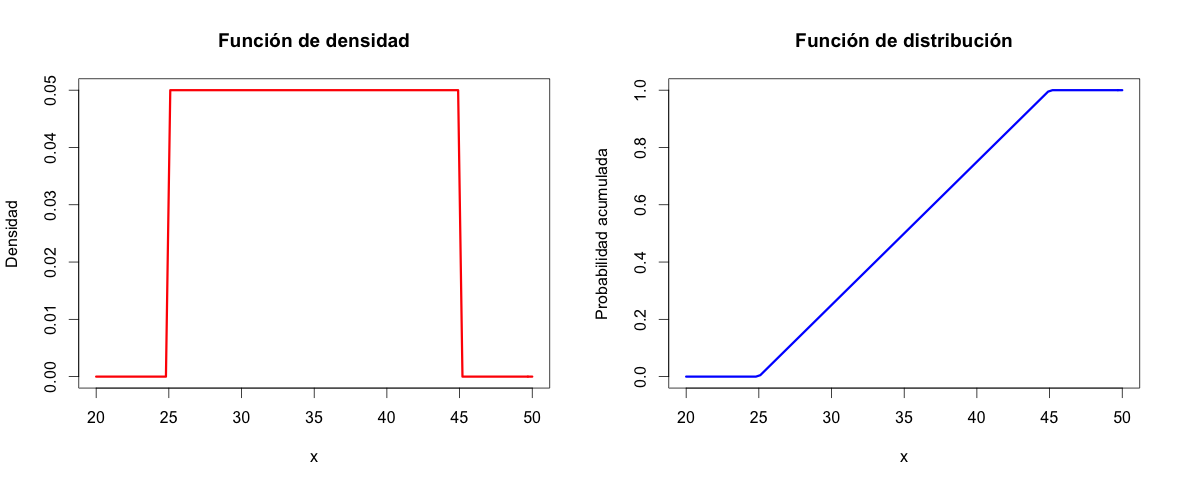
\includegraphics[width=0.9\linewidth]{imagenes/funcion_distribucion_uniforme}
\caption{Funciones de densidad y distribución de la distribución uniforme}
\label{fig:funcion_distribucion_uniforme}
\end{figure}

La esperanza de una de una distribución uniforme de parámetros $(a, b)$ viene dada por

\begin{align*}
E[X] & = \dfrac{a + b}{2}\\
Var[X] & = \dfrac{(b-a)^2}{12}
\end{align*}

Haciendo $a = 25$ y $b = 45$, se tiene que

\begin{align*}
E[X] & = \dfrac{25+45}{2} = 35\\
Var[X] & = \dfrac{(45-25)^2}{12} = \dfrac{100}{3}
\end{align*}

La probabilidad de que $X$ sea, como mucho, 30 minutos es $P(X \leq 30)$.\\

\begin{align*}
P(X \leq 30) & = \int_{25}^{30} \dfrac{1}{45 -25} \ dx \\
& = \dfrac{1}{20}\left[x\right]_{25}^{30} \\ & = \dfrac{1}{4}
\end{align*}

La probabilidad de que $X$ esté comprendido entre 30 y 40 minutos es $P(30 \leq X \leq 40)$.\\

\begin{align*}
P(30 \leq X \leq 40) & = \int_{30}^{40} \dfrac{1}{45 -25} \ dx \\
& = \dfrac{1}{20}\left[x\right]_{40}^{30} \\ & = \dfrac{1}{2}
\end{align*}

Calculamos el percentil 90 de la distribución. Es decir tenemos que encontrar el número $a$ tal que acumula el 90\% de la probabilidad. Es decir,

\begin{align*}
\int_{25}^{a} \dfrac{1}{45 - 25} \ dx = 0.9
\end{align*}

\begin{align*}
\dfrac{1}{20}\int_{25}^{a} dx = \dfrac{1}{20} \left[x\right]_{25}^{a} = \dfrac{1}{20}(a - 25) = 0.9
\end{align*}

Despejando $a$ se tiene que $a = 0.9 \cdot 20 + 25 = 43$.\\

Es decir, el 90\% de las tartas llegará en un tiempo menor o igual a 43 minutos.\\

La probabilidad de que el tiempo $X$ sea mayor de 40 minutos sabiendo que dicho tiempo es de al menos 30 minutos es $P(X > 40 | X > 30)$.

\begin{align*}
\displaystyle P(X > 40 | X > 30) & = \dfrac{P(\{X > 40\}\cap \{X > 30\})}{P(X > 30)} \\
& = \dfrac{P(X > 40)}{P(X > 30)} \\ & = \dfrac{1 - P(X \leq 40)}{1 - P(X \leq 30)} \\
& = \dfrac{1 - \displaystyle \int_{25}^{40} \dfrac{1}{20} \ dx}{1 - \displaystyle \int_{25}^{30} \dfrac{1}{20} \ dx} \\
& = \dfrac{1 - \dfrac{1}{20}(40-25)}{1 - \dfrac{1}{20}(30-25)} \\
& = \dfrac{1- \dfrac{3}{4}}{1 - \dfrac{1}{4}} \\
& = \dfrac{1}{3}
\end{align*}

Por tanto, sabiendo que el tiempo de llegada de las tartas va a ser mayor de 30 minutos, tenemos un 33.33\% de probabilidades de que tarden más de 40 minutos.

\subsection{Tarea VII}

Si ahora denotamos con $X$ al tiempo (en minutos) que dura una llamada cualquiera realizada por un trabajador de VACIS a un teléfono externo, tenemos que $X \sim \mathcal{E}xp(\lambda)$. Se sabe que la duración media de una llamada es de 8 minutos.\\

Así pues, sabemos que $E[X] = \dfrac{1}{\lambda}$. Por otro lado, tenemos que la duración media de las llamadas es de 8 minutos, es decir, $E[X] = 8$. Si igualamos y despejamos $\lambda$ tenemos que $\lambda = \dfrac{1}{8}$. Por tanto, $X \sim \mathcal{E}xp\left(\dfrac{1}{8}\right)$. La Figura~\ref{fig:funcion_distribucion_exponencial} muestra tanto la función de densidad como la de distribución de esta variable aleatoria.\\

\begin{figure}[tbph!]
\centering
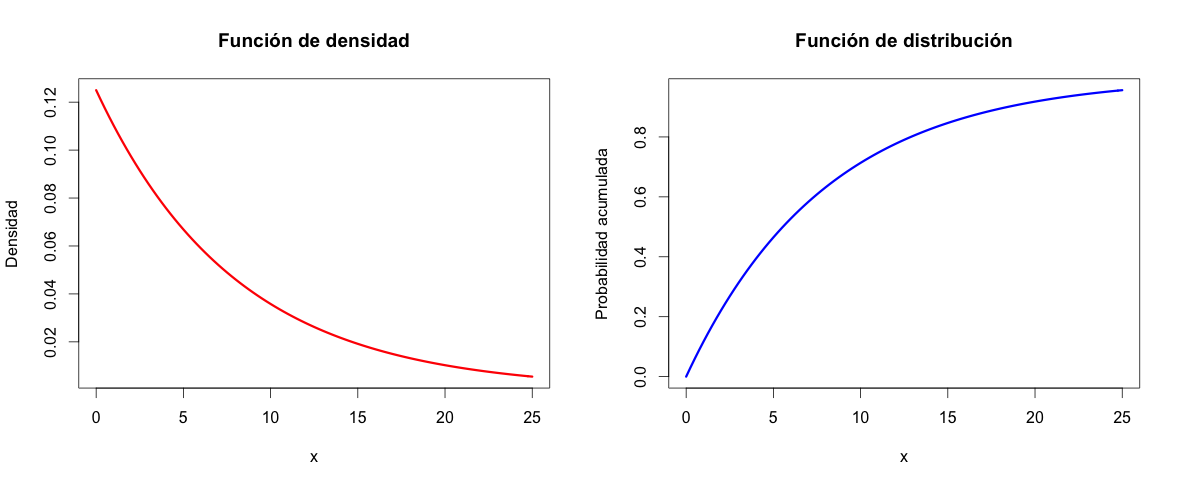
\includegraphics[width=0.9\linewidth]{imagenes/funcion_distribucion_exponencial}
\caption{Funciones de densidad y distribución de la distribución exponencial}
\label{fig:funcion_distribucion_exponencial}
\end{figure}

La esperanza y la varianza de una distribución exponencial con parámetro $\lambda$ viene dada por

\begin{align*}
E[X] & = \dfrac{1}{\lambda} \\
Var[X] & = \dfrac{1}{\lambda^2}
\end{align*}

Sustituyendo $\lambda  = \dfrac{1}{8}$, tenemos que

\begin{align*}
E[X] & = \dfrac{1}{\dfrac{1}{8}} = 8 \\
Var[X] & = \dfrac{1}{\left(\dfrac{1}{8}\right)^2} = 64
\end{align*}

La probabilidad de que una llamada cualquiera a móvil dure menos de 9 minutos es $P(X < 9)$,

\begin{align*}
P(X < 9) & = \int_{0}^{9} \dfrac{1}{8} e^{-\dfrac{x}{8}} \ dx \\
& = -\left[ e^{-\dfrac{x}{8}} \right]_0^9 \\
& = 1 - e^{-\dfrac{9}{8}} \\
& = 0.675
\end{align*}

La probabilidad de que una llamada cualquiera a móvil dure entre 7 y 9 miutos es $P(7 \leq X \leq 9)$,

\begin{align*}
P(7 \leq X \leq 9) & = \int_{7}^{9} \frac{1}{8} e^{-\frac{x}{8}} \ dx \\
& = -\left[ e^{-\frac{x}{8}} \right]_7^9 \\
& = -e^{-\frac{9}{8}} + e^{-\frac{7}{8}} \\
& = 0.092
\end{align*}

Calculamos el percentil 80 de esta distribución, es decir, el número $a$ tal que la probabilidad acumulada de la distribución es del 80\%. Es decir,

\begin{align*}
\int_{0}^{a} \frac{1}{8} e^{-\frac{x}{8}} \ dx = 0.8
\end{align*}

\begin{align*}
\int_{0}^{a} \frac{1}{8} e^{-\frac{x}{8}} \ dx & = - \left[ e^{-\frac{x}{8}} \right]_0^a \\
& = -e^{\frac{a}{8}} + 1 \\
& = 0.8
\end{align*}

Tomando logaritmos a ambos lados de la expresión anterior, se tiene que 

\begin{align*}
a = -8 \cdot \ln 0.2 = 12.875
\end{align*}

Por tanto, el 80\% de las llamadas tienen una duración inferior a 12.875 minutos.\\

Si tenemos un total de 1000 llamadas a móvil al día, el tiempo total de esas llamadas es de 8000 minutos diarios, ya que la duración media de una llamada cualquiera es de 8 minutos. Así 1000 llamadas $\cdot$ 8 minutos/llamada = 8000 minutos. Si queremos ser más precisos, con nuestra estimación podemos calcular un intervalo de probabilidad al 90\%.\\

Normalmente, calculamos los intervalos de probabilidad bilaterales, pero en este caso, por tratarse de una distribución con alta asimetría hacia la derecha, calcularemos el intervalo con los percentiles 0 y 0.90. Si calculamos estas probabilidades como en el apartado anterior tenemos que el intervalo es $(0, 18.42)$ (Figura~\ref{fig:intervalo_probabilidad_exponencial}). Es decir, el 90\% de las llamadas estarán entre 0 y 18.42 minutos. Por tanto, el número de minutos a diario estará entre 0 y 18420 minutos diarios.\\

\begin{figure}[tbph!]
\centering
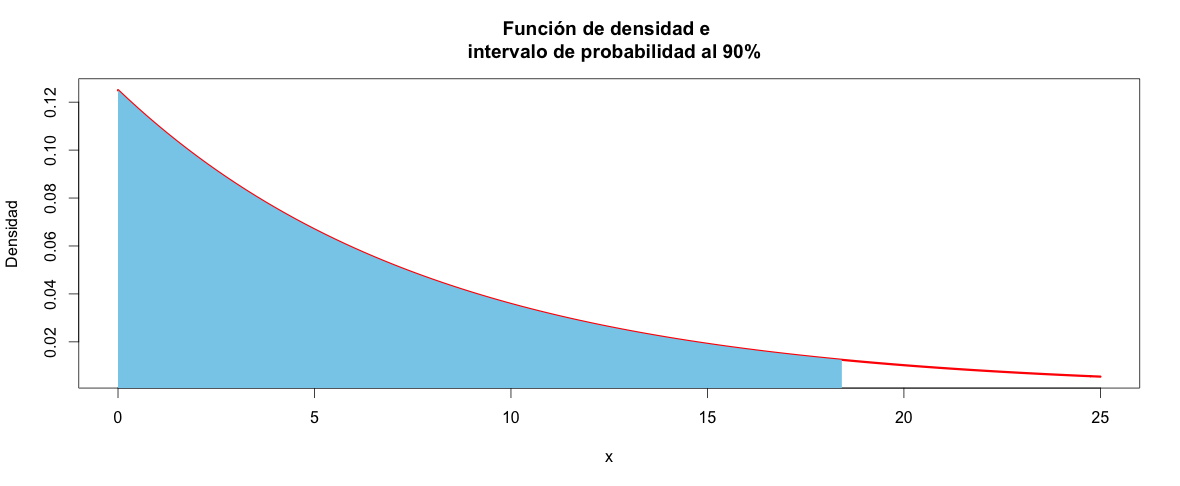
\includegraphics[width=0.9\linewidth]{imagenes/intervalo_probabilidad_exponencial}
\caption{Funciones de densidad e intervalo de probabilidad al 90\% de la distribución exponencial}
\label{fig:intervalo_probabilidad_exponencial}
\end{figure}

Si nuestra tarifa móvil actual (en minutos) es:

\begin{align*}
Y = \begin{cases}
0.1 + 0.6X & \text{si } X < 1 \\
0.1 + 0.3X & \text{si } X \geq 1
\end{cases}
\end{align*}

El coste medio de esta nueva variable aleatoria viene dado por su esperanza,

\begin{align*}
E[Y] = \begin{cases}
0.1 + 0.6E[X] & \text{si } X < 1 \\
0.1 + 0.3E[X] & \text{si } X \geq 1
\end{cases} = \begin{cases}
4.9 & \text{si } X < 1 \\
2.5 & \text{si } X \geq 1
\end{cases}
\end{align*}

Por otro lado, la probabilidad de tener una llamada de menos de un minuto es de 11.7\%, y tener una llamada superior a un minuto es de 88.3\%. Usamos estas probabilidades para ponderar el coste medio de una llamada.\\

\begin{align*}
E[Y] & = 0.117 \cdot 4.9 + 0.883 \cdot 2.5 \\
& = 2.7808
\end{align*}

Por tanto, el coste medio para una llamada es de 2.78€. Si se realizan 1000 llamadas el coste es de 2780€.\\

Para calcular la varianza, procedemos como con la esperanza.\\

\begin{align*}
Var[Y] = \begin{cases}
0.6^2 \cdot Var[X] & \text{si } X < 1 \\
0.3^2 \cdot Var[X] & \text{si } X \geq 1
\end{cases} = \begin{cases}
23.04  & \text{si } X < 1 \\
5.76 & \text{si } X \geq 1
\end{cases}
\end{align*} 

Ponderando como con la media se obtiene que $Var[Y] = 7.781$. Por tanto, la desviación típica es $2.789$\\

Si repetimos lo anterior, pero haciendo una simulación, es decir, generamos 1000 muestras de una distribución exponencial con parámetro $\lambda = \dfrac{1}{8}$. Aplicamos nuestra función de coste a cada una de nuestras muestras, y calculamos la media y la varianza. En nuestro caso, el coste medio por llamada es de 2.601€, el coste total es de 2601.67€ y la desviación típica es de 2.530€. La Figura~\ref{fig:simulacion} muestra la duración y el coste de las 1000 llamadas simuladas.\\

\begin{figure}[tbph!]
\centering
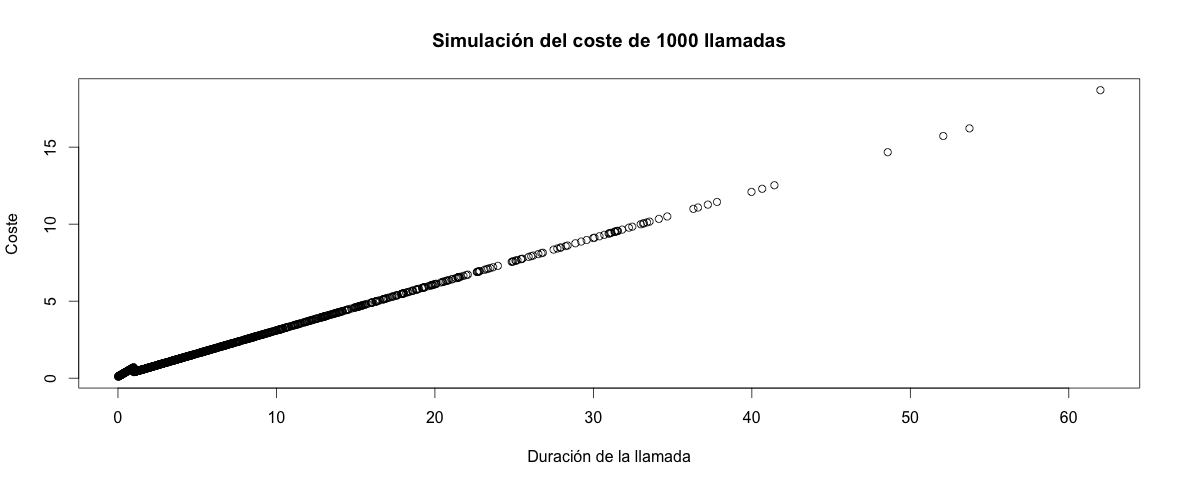
\includegraphics[width=0.9\linewidth]{imagenes/simulacion}
\caption{Simulación del coste de 1000 llamadas}
\label{fig:simulacion}
\end{figure}

\section{Conclusiones}

En esta actividad hemos puesto en práctica lo aprendido en teoría sobre variables aleatorias --tanto continuas como discretas-- y cálculo de probabilidades, y hemos aplicado estas variables aleatorias para modelizar distintos tipos de problemas. R nos ha permitido calcular probabilidades y representar gráficos de forma rápida, ahorrándonos una gran cantidad de tiempo. 

\newpage

\section{Código R}

\verbatiminput{../caso_ii2.0.R}


\end{document} 